% !TeX spellcheck = fr_FR
\chapter{Chapitre 0 : Base Technique}

Ce chapitre a pour but d'introduire et expliquer les différents aspects techniques clés de ce projet de semestre. Je vais notamment expliquer brièvement ce qu'est un \gls{fpga} et le principe d'une fonction de hachage.

\section{FPGA}
Un \gls{fpga} est un \gls{ic} dans lequel on peut programmer et interconnecter des circuits logiques. Contrairement à un processeur, qui est limité par un certain nombre d'instructions et exécute les instructions de manière séquentielle, un FPGA permet d'exécuter de nombreux circuits logiques en parallèle.

Pour programmer un \gls{fpga}, on utilise généralement des langages de description matériel tels que le \gls{vhdl} et le Verilog. Dans ce projet, j'ai personnellement travaillé avec le \gls{vhdl}.

Lorsque l'on souhaite tester un programme \gls{vhdl}, il est possible d'utiliser des outils de simulation afin de vérifier le fonctionnement souhaité. Il est aussi possible d'automatiser la phase de simulation à l'aide de fichier que l'on appelle testbench.

Durant ce travail, j'ai utilisé Vivado qui est le logiciel qui m'a permis la simulation et la programmation des \gls{fpga} qui ont été utilisés. 
\section{Fonction de hachage}

Une fonction de hachage est une fonction qui va prendre en entrée une donnée a taille variable et va ressortir une donnée de taille fixe. 

Une des propriétés fondamentales d'une fonction de hachage est qu'il n'existe pas de fonction mathématique permettant de retrouver la donnée originale à partir d'un hash généré. 
Même une petite modification apportée à la donnée en entrée conduira à un hash totalement différent en sortie. 
Cette particularité est essentielle pour sécuriser le stockage des mots de passe, car même si des hash venait à être compromises, il est extrêmement difficile de retrouver les mots de passe originaux à partir de leurs hachages.

\newpage

\begin{figure}[tbph!]
	\centering
	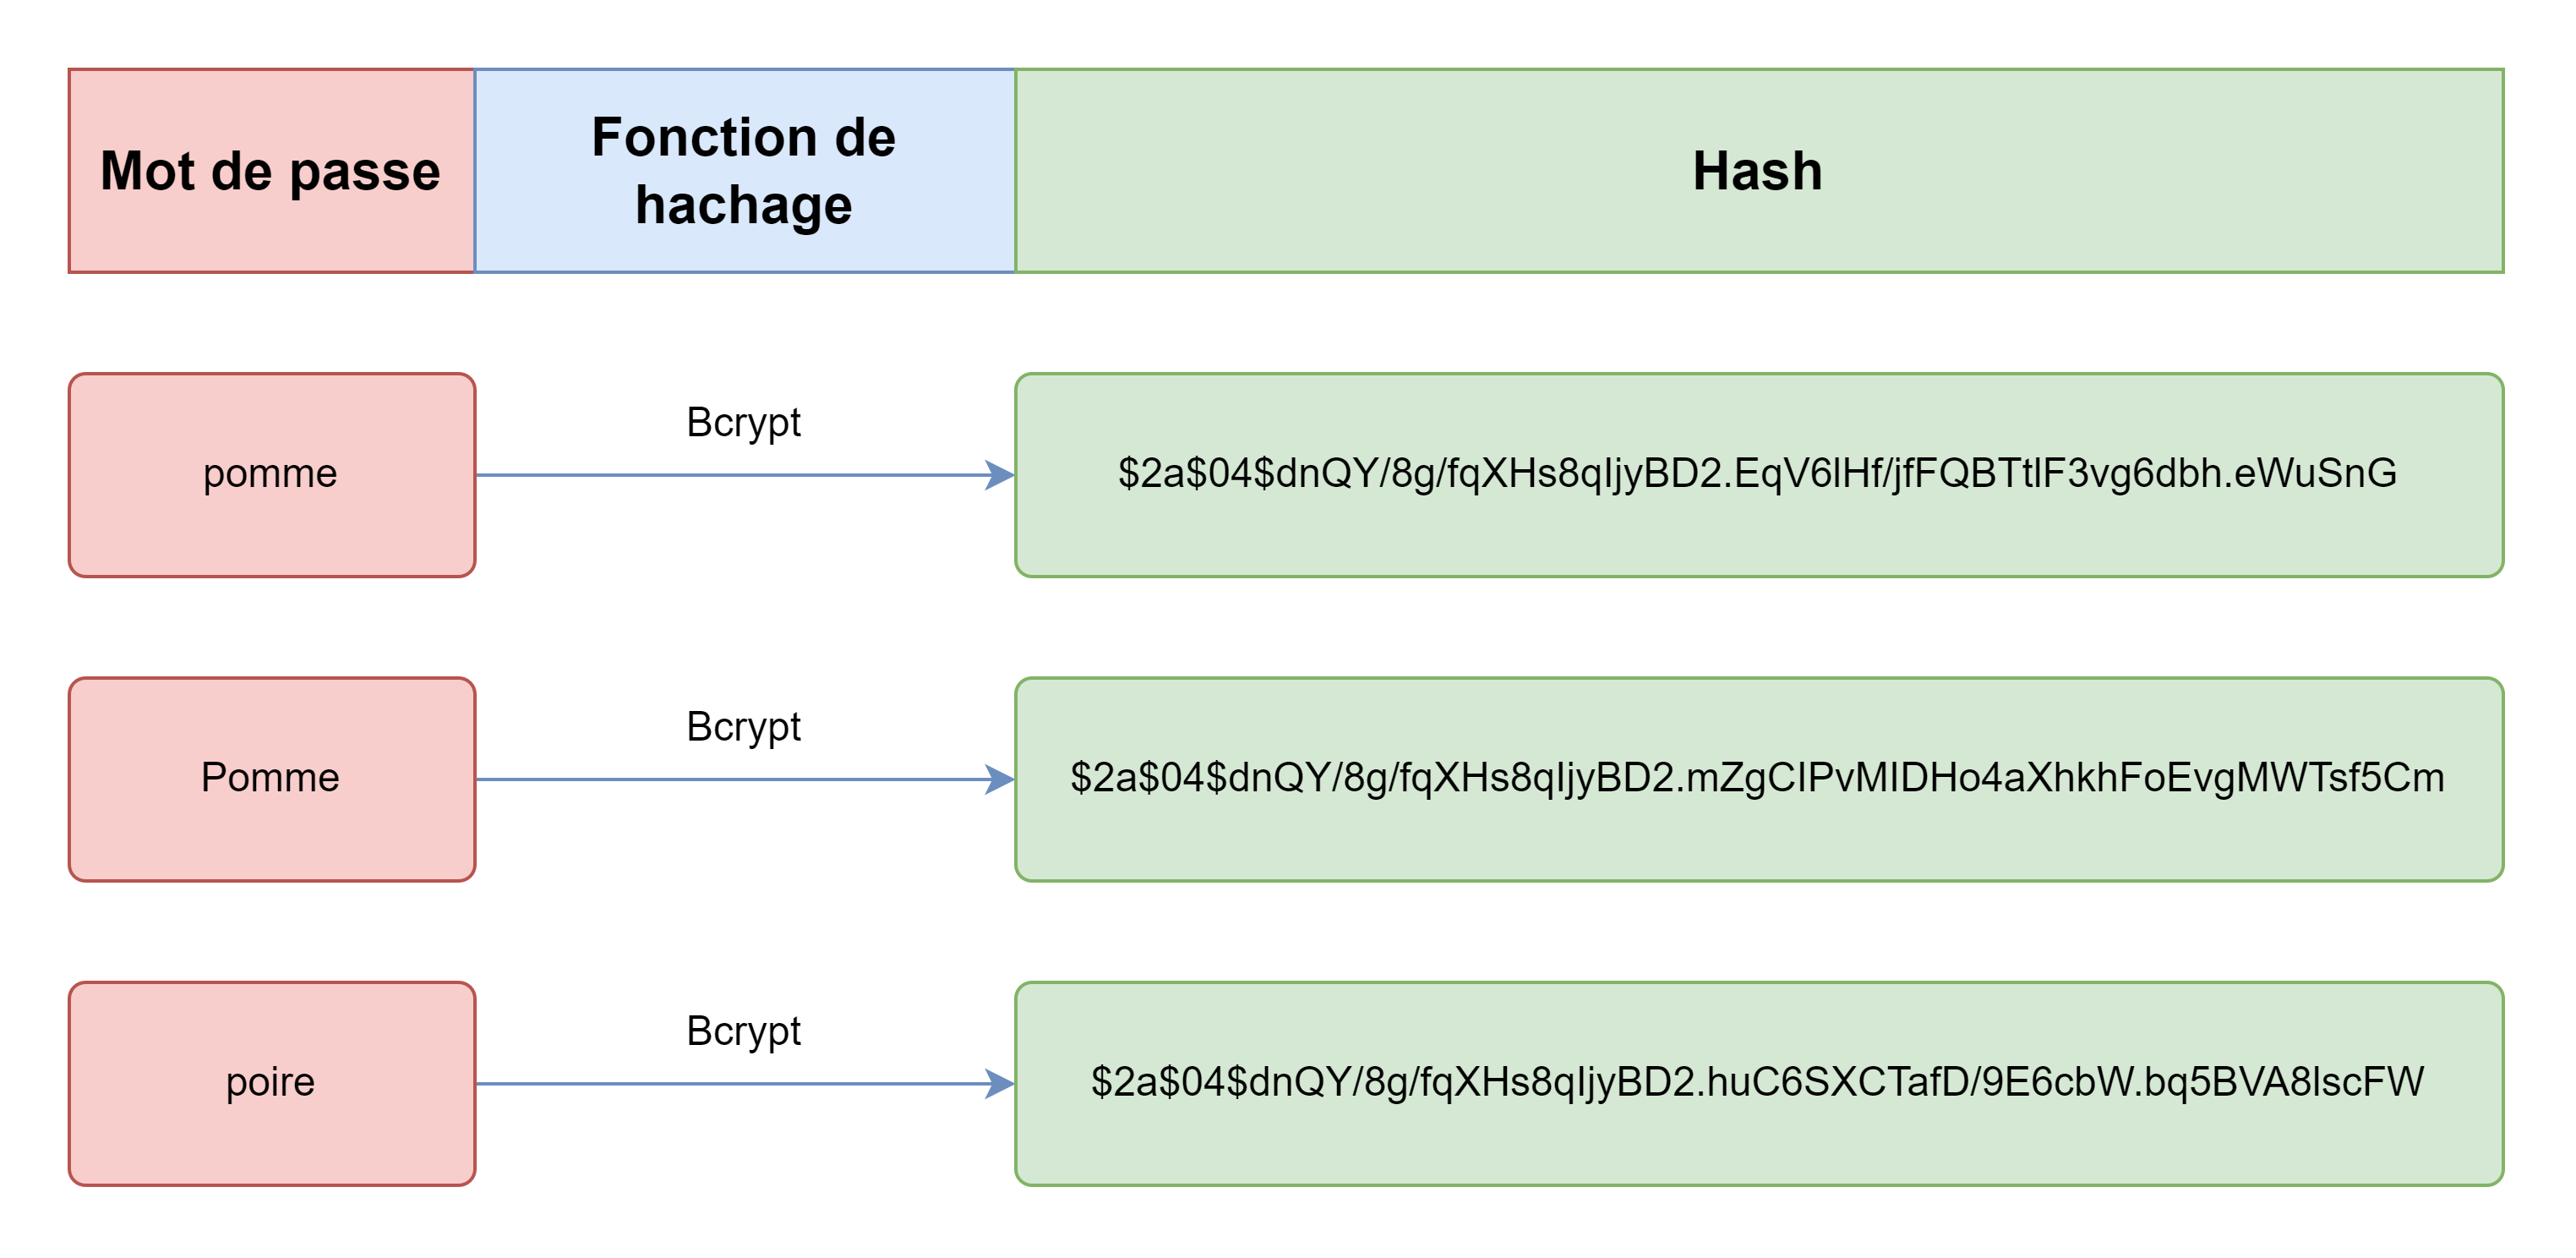
\includegraphics[width=0.7\linewidth]{hash_function}
	\caption[Fonction de hachage]{Fonction de hachage. Source : réalisé par Kandiah Abivarman}
	\label{fig:fonction_hachage}
\end{figure}


\subsection{Salt}

Certaines fonctions de hachage tel que le bcrypt utilisent ce qu'on appelle un salt (sel en français), qui est une valeur générée aléatoirement qu'on va donner avec notre mot de passe. Le salt va permettre d'avoir un hash différent, même si deux personnes utilisent le même mot de passe, ajoutant ainsi une couche supplémentaire de sécurité.

\begin{figure}[tbph!]
	\centering
	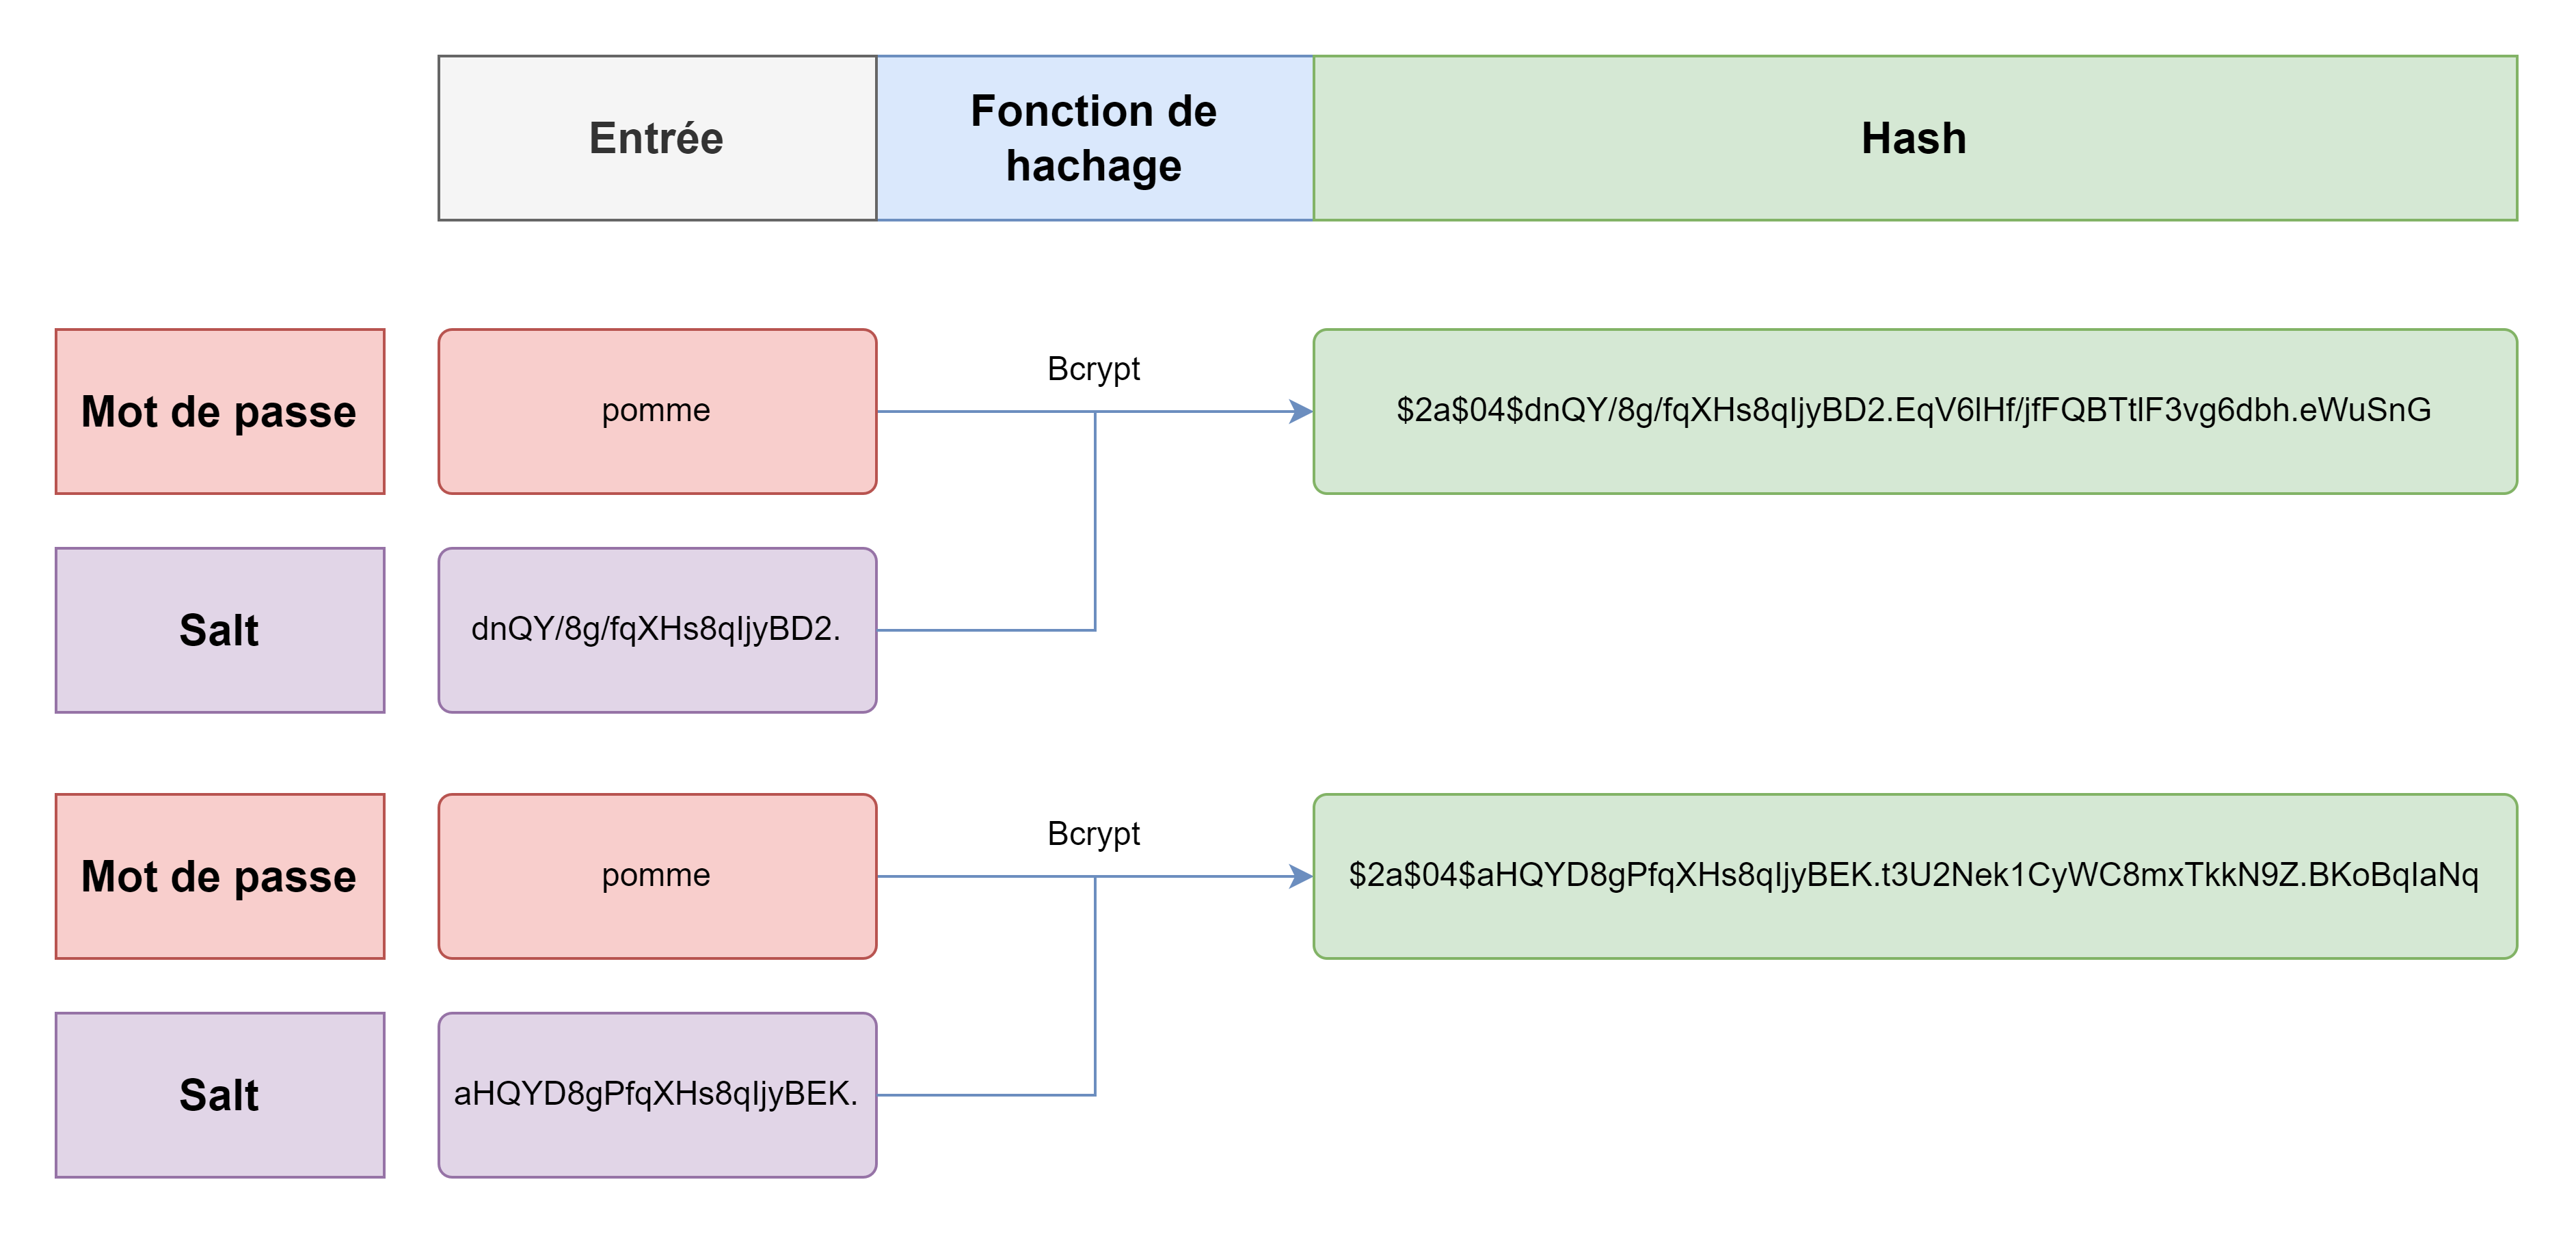
\includegraphics[width=0.7\linewidth]{hash_salt}
	\caption[Salt]{Salt. Source : réalisé par Kandiah Abivarman}
	\label{fig:hash_salt}
\end{figure}

\newpage

\subsection{Attaque par bruteforce}

L'attaque par bruteforce consiste à essayer toutes les combinaisons possibles de mots de passe afin de retrouver celui qui correspond au hash compromis. Cette méthode repose sur le fait qu'il est impossible de retrouver directement le mot de passe à partir du hash, obligeant ainsi l'attaquant à tester différentes entrées jusqu'à ce qu'il trouve celle qui génère le hash recherché.

Toutefois, cette méthode peut prendre beaucoup de temps, notamment lorsque les fonctions de hachage utilisées sont conçues pour être lentes à calculer.